\documentclass[conference]{IEEEtran}
\usepackage{bm}
\usepackage{cite}
\usepackage{ragged2e}
\usepackage{graphicx}
\usepackage{amsmath}
\usepackage{amssymb}
\usepackage{amsthm}
\usepackage{algorithm}
\usepackage{algpseudocode}
\usepackage{enumitem}
\usepackage{etoolbox}
\usepackage{mathrsfs}
\usepackage{subfig}
\usepackage{array}
\usepackage{cases}
\usepackage{dsfont}
\usepackage{optidef}
\usepackage{cleveref}

\allowdisplaybreaks
\newtheorem{theorem}{Theorem}
\newtheorem{lemma}{Lemma}
\newtheorem{definition}{Definition}
\setlength{\columnsep}{0.21in}
\makeatletter
\newcommand\fs@betterruled{%
  \def\@fs@cfont{\bfseries}\let\@fs@capt\floatc@ruled
  \def\@fs@pre{\vspace*{0.03in}\hrule height.8pt depth0pt \kern2pt}%
  \def\@fs@post{\kern2pt\hrule\relax}%
  \def\@fs@mid{\kern2pt\hrule\kern2pt}%
  \let\@fs@iftopcapt\iftrue}
\floatstyle{betterruled}
\restylefloat{algorithm}
\makeatother
\renewcommand{\arraystretch}{1.2}
\begin{document}
\title{Final Report for Wireless Mobile Network}
\author{\IEEEauthorblockN{Chia-Hung Lin, Chun-Yen Lee, Lu-Yo Kuo}
\IEEEauthorblockA{
Department of Electrical Engineering, National Taiwan University \\
b06504016@ntu.edu.tw, b06203017@ntu.edu.tw, b06502153@ntu.edu.tw
}}
\maketitle
\begin{abstract}
The abstract goes here.
\end{abstract}

\section{Introduction}
To be added
\section{HW5}
\subsection{System Model}
The system is about Device to Device (D2D) systems. The distance between receive and transmission pair is fixed to $100m$. Both transmission user equipment (UE) and receive UE are in the central cell. There are $75$ UE pairs in the system.
\begin{figure}[htbp]
    \centering
    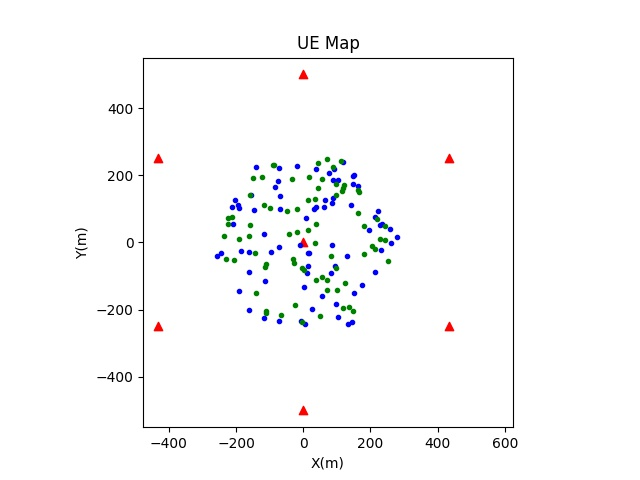
\includegraphics[width=0.45\textwidth]{fig1_1.jpg}
    \caption{The simulated map for UEs}
    \label{fig:ue_map}
\end{figure}


In \Cref{fig:ue_map}, the green point indicates the receive UE, and the blue point indicates the transmission UE. The red triangle indicates the base stations in the system.  
\subsection{Basic D2D Topology Simulation}
\subsubsection{Simulation Parameters}
In the system, the bandwidth is $10$MHz, the temperature is $27^\circ$C, the power of the base stations is $23$dBm, the power of UEs in $0$dBm, the antenna gain of receive and transmit is both $0$dB. The UE height is $1.5$m, and the base station height is $51.5$m. The path loss model is Two-ray-ground model, which can be written as
\begin{equation}\label{eqn:two_ray}
    g(d) = P_t \times \dfrac{Gh_t^2h_r^2}{d^4}
\end{equation}
where $P_t$ is the transmit power, and $G$ is the total gain, $h_t$ and $h_r$ are height of transmit and receive antennas respectively.
\subsubsection{PMF for Uplink SINR}
In uplink scenario, as shown in \Cref{fig:uplink_sinr}, the SINR of the uplink signal is between $60$ to $100$ dB, which is very large. This can be explained by the assumption that there is no interference in the uplink transmission. 
\begin{figure}[htbp]
    \centering
    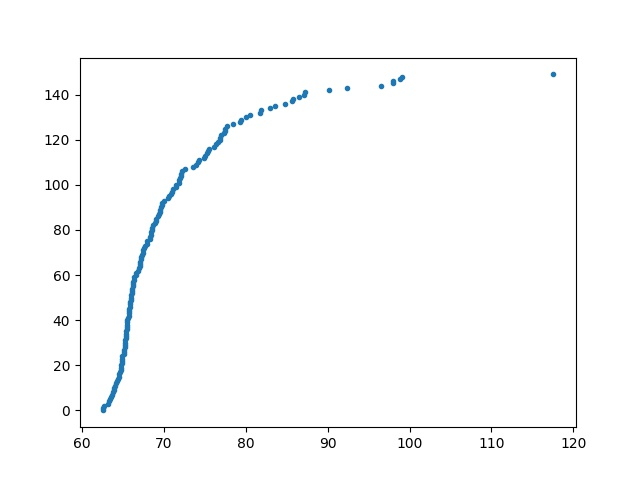
\includegraphics[width=0.45\textwidth]{fig1_2_a.jpg}
    \caption{PMF for Uplink SINR}
    \label{fig:uplink_sinr}
\end{figure}

\subsubsection{PMF for Downlink SINR}
In downlink scenario, as shown in \Cref{fig:downlink_sinr}, the SINR of the downlink signal is between $0$ to $50$ dB. 


\begin{figure}[htbp]
    \centering
    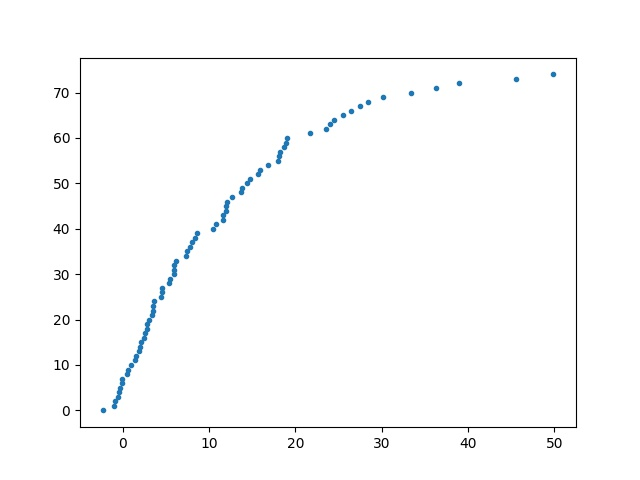
\includegraphics[width=0.45\textwidth]{fig1_2_b.jpg}
    \caption{PMF for Downlink SINR}
    \label{fig:downlink_sinr}
\end{figure}
Although the power of the downlink is from the base station, the SINR is smaller than the uplink signal. The difference is mainly cause by the different presumption of the uplink and downlink transmission signal, where the uplink signal is hypothesized to be interference-free, and the downlink signal is assumed to be interference by the signal from other base station.
\subsubsection{Total Throughput of the Downlink transmission}
By the simulation, the total throughput is approximately $2.43$ Gbps.
\subsubsection{PMF of the D2D SINR}

\begin{figure}[htbp]
    \centering
    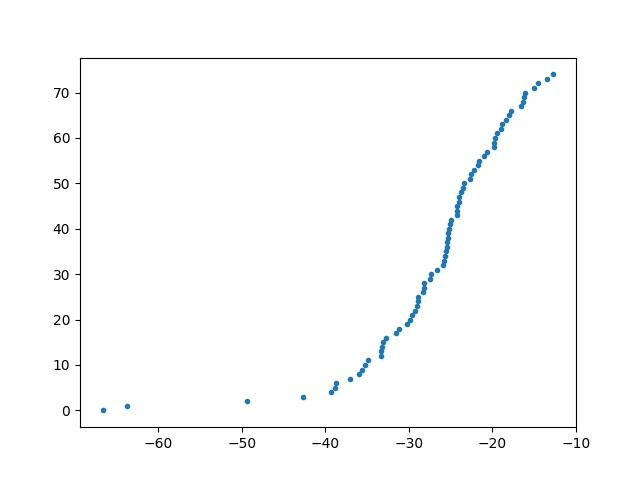
\includegraphics[width=0.45\textwidth]{fig1_4.jpg}
    \caption{PMF for D2D SINR}
    \label{fig:d2d_sinr}
\end{figure}
In D2D system, as shown in \Cref{fig:d2d_sinr}, the SINR of the D2D signal is mostly between $-60$ to $-10$ dB. 
\subsubsection{Total Throughput of the D2D system}
By the simulation, the total throughput is approximately $9.98$ Mbps.
\subsubsection{Total Throughput with different number of D2D pairs}
\begin{figure}[htbp]
    \centering
    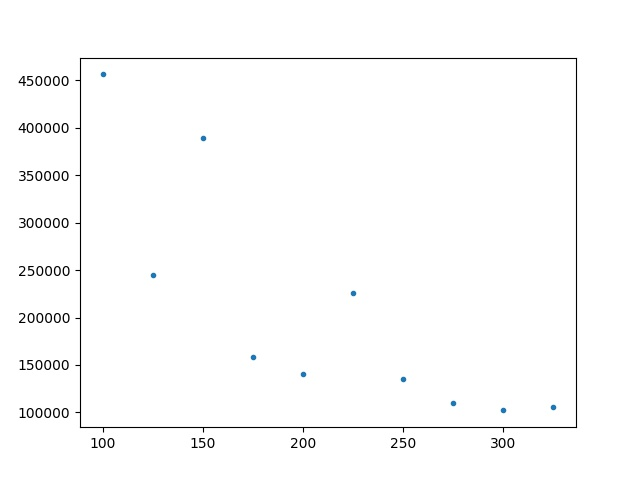
\includegraphics[width=0.45\textwidth]{fig1_6.jpg}
    \caption{Total Throughput vs. Number of D2D Pair}
    \label{fig:d2d_num}
\end{figure}
\subsection{Traffic in D2D Simulation}
\subsubsection{Bit Loss Probability in UL and DL system}
\subsubsection{Bit Loss Probability in D2D system}
\section{HW6}
\subsection{System Model}
\subsection{Simulation}
\section{Conclusion}
The conclusion goes here.
\end{document}


